\documentclass{article}
\usepackage{graphicx}
\usepackage{fancyhdr}
\pagestyle{fancy}

%=====================================================
% macros

\newcommand{\libfadc}{\emph{\texttt{libfadc}} }
\newcommand{\F}[1]{\texttt{#1}}
\newcommand{\testfadc}{\emph{TestFADC} }

%=====================================================

\begin{document}

  \title{\testfadc 1.x Users Guide}
  \author{Karl Kosack}
  \maketitle
  \tableofcontents
  \newpage

\section{Introduction}

\testfadc is a simple program which allows one to view in real-time the
output of an FADC board.  Much like a digital oscilloscope,
\testfadc also makes a variety of measurements for each pulse
(e.g. width, rise time, area, etc.), produces histograms, and can save
individual waveforms and data for processing in other programs.

\testfadc started out as my first attempt at communicating with an
FADC board in QNX, and was not originally intended to be a useful
program.  However, it turned out to be easier to add features to it
than my more fancy data acquisition programs, and was \emph{much}
easier to port to Linux (I had used POSIX real-time extensions for the
other software, which are not yet supported in Linux).  In the end,
\testfadc ended up becoming a very useful tool, though the interface
is a bit rough around the edges and it's certainly not elegant. I'm
currently working on \testfadc 2.0, a completely re-written version in
C++ with Qt widgets and a faster event-grabbing core, but it may be a
while before it is as stable as the current version.  In this
document, I will attempt to explain how to use efficiently all the
various features of \testfadc 1.0.

%=================================================================
\section{Running \testfadc}

To start the program, simply type '\F{testfadc -bN}', where \F{N} is
the number of the FADC board you want to use.  \testfadc can also take
a '\F{-t}' switch which turns off the graphical dialog boxes and uses
the console to ask for user input.  The reason for this is I've
noticed that there is a bug in the libsx X widget library on certain
servers where sometimes the text fields in the dialog boxes are not
editable (even though they should be). If you notice this happening,
run '\F{testfadc -t -b1}' instead. Note that when you choose an option
from the "SET" menu, you will see a text prompt for an answer on the
terminal where you started testfadc instead of popping up in a
dialog. That's a kind of ugly solution, but it works.  It won't be a
problem in the Qt version.

When \testfadc loads, it looks for a file in the current directory
called \F{fadc-board-N.settings} (where \F{N} is the board number),
which is a \libfadc board settings file. It that file exists, all the
board parameters will be loaded from it; otherwise the defaults will
be used (see \libfadc documentation).  You can use \testfadc to
generate such a file (see ``Save Current Settings...'' in Section
\ref{savesettings}).

%=================================================================
\section{The Interface}

\begin{figure}
  \begin{center}
    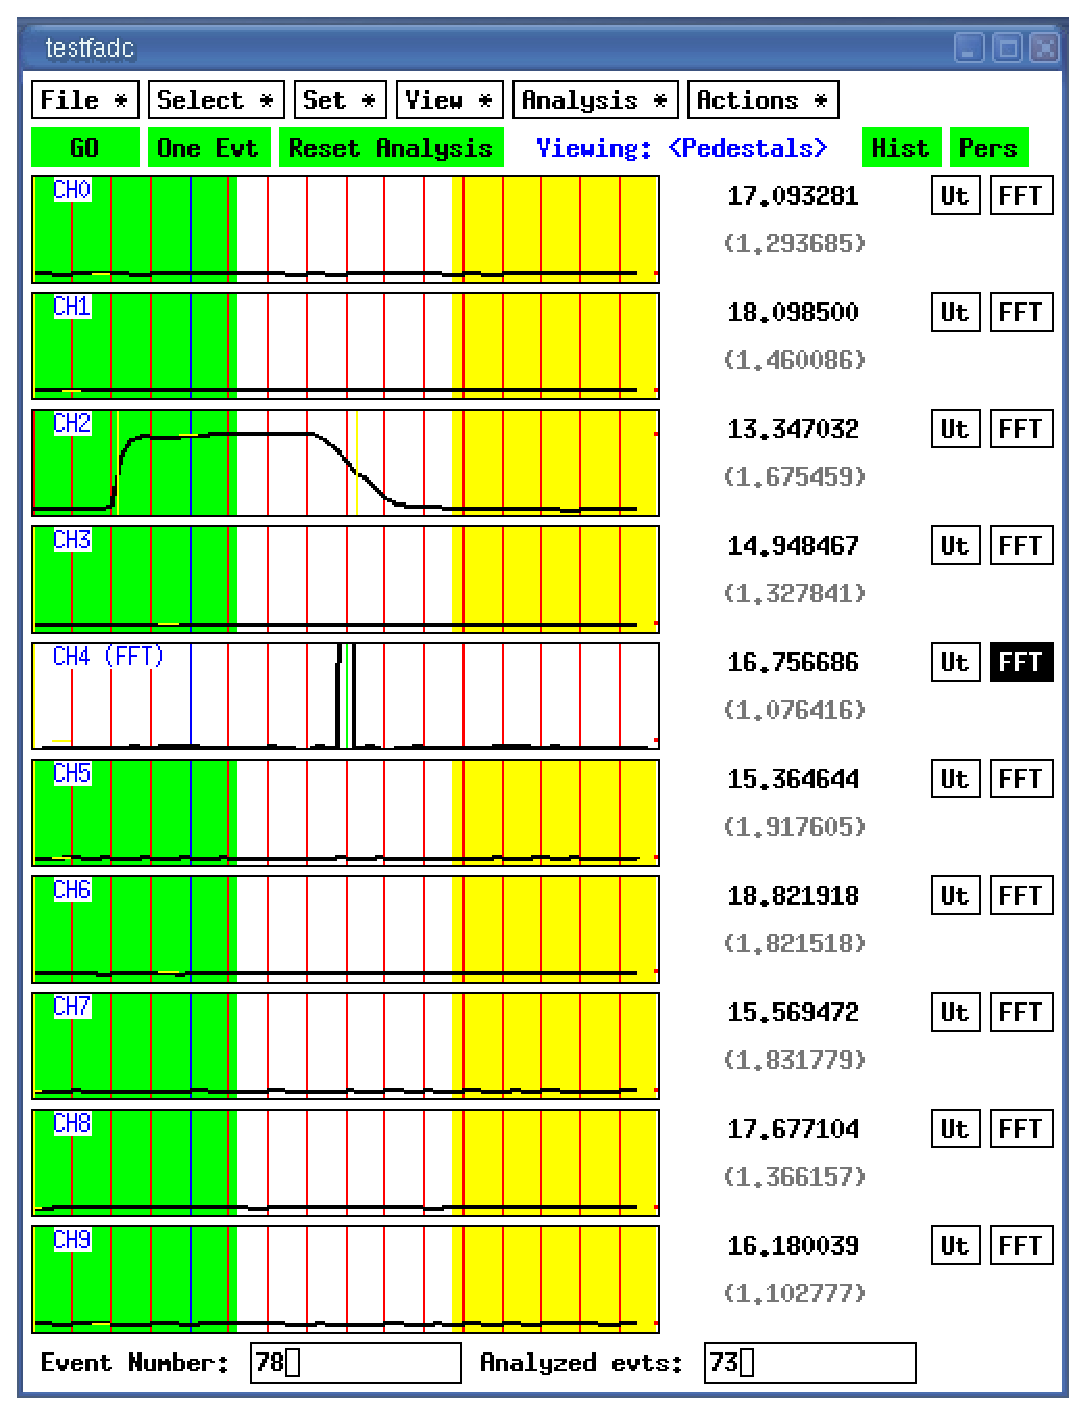
\includegraphics[width=10cm]{testfadc-screenshot.eps}
    \caption{Screenshot of \testfadc in action}
  \end{center}
\end{figure}


%-------------------------------------------------
\subsection{Button Bar}
\subsubsection{GO/STOP}
Press this button to continuously grab events for graphics display and
analysis.

\subsubsection{One Evt}
Only grab one event at a time (for each press). Also dumps
the parsed data from the event to the console for debugging.

\subsubsection{Reset Analysis}
Sets all cumulative measurement averages and histograms to zero.

\subsubsection{Hist}
This toggles the on-screen peak histogram display.  The peak histogram for
each channel will be plotted on the far right of each waveform
display. Many other histograms are generated, but the others must be
viewed with an external program (like \F{gnuplot}).  See ``Write
Histograms'' in Section \ref{writehist} for more information. 

\subsubsection{Pers}

Toggles the ``persistent'' display of waveforms (waveforms are plotted
over each other and not erased).  This is useful for looking at the
time jitter.

%-------------------------------------------------
\subsection{Waveform Displays}

The center of the \testfadc window contains the waveform views, one
for each channel. These display the waveforms for the current event.
The peak position and height for each pulse is displayed as a yellow
tick mark on the waveform.  A vertical red bar is plotted every 4
samples (which corresponds to 8 ns).

\subsubsection{Disabling}

Click a waveform display with the RIGHT mouse button to disable that
channel on the FADC.  

\begin{quote}
\textbf{NOTE}: When you are using "Acquire Data" mode (see below), you
may want to disable all channels except the one(s) which have
pulses to reduce the amount of data written to the disk. Data
is only returned for channels which are enabled. This is also
useful when using the "One Evt" button, so the data written to
the console is not overwhelming.
\end{quote}


\subsubsection{Selecting}

Click a waveform display with the LEFT mouse button to select or
unselect that channel (by default all channels are selected).  Options
in the ``Set'' and ``Analysis'' menus  apply only to the selected
channels. See the ``Select'' menu documentation for more info.

\subsubsection{Zooming}

Click with the  mouse button to zoom in on the channel.  Note: the
zoom windows do not automatically update in "GO" mode. 

\begin{quote}
  \textbf{IMPORTANT}: when a Zoom window is open, push the "close" button
  in the lower left-hand corner to close it!  If you use the
  window manager's close button to close the window, all of
  testfadc will exit!  I'll try to fix that in a later release.
\end{quote}


%-------------------------------------------------
\subsection{Measurement Display}

To the right of each waveform display, the measurement currently
selected in the ``View'' menu  is displayed.  For average
measurements, there are two numbers, the average value is on top and
the dispersion is on the bottom (in parentheses).

%-------------------------------------------------
\subsection{CFD buttons}

To the right of each measurement display is a button which toggles \testfadc
between using a Washington University CFD interface (WU) vs. a University
of Utah CFD interface for that channel (Ut).  Channels with WU set
respond to the ``wuthresh'' and ``wuoffs'' commands in the ``Set''
menu, while the Ut channels respond to the ``threshold'' and
``ratefb'' settings.

%-------------------------------------------------
\subsection{FFT buttons}

Toggling the ``FFT'' buttons to the right of each measurement display
will cause the fourier transform of the waveform to be displayed
instead of the time-domain pulse.  This feature only works when the
Datawidth of the board is set to a power of 2 (and is disabled
otherwise).

%-------------------------------------------------
\subsection{Menus}

%-------------------------------------------------
\subsubsection{File}
\paragraph{About...}
Show an about message. Pretty standard.


\paragraph{Save Current Settings...}
\label{savesettings}
Write all of the current FADC and CFD settings into a \libfadc
settings text file, so that they can be loaded later (automatically at
startup).

\paragraph{Save Waveforms...}
Asks for a file-name base (like "pulse-dump") and writes the currently
displayed pulses into tab-delimited data files for each channel
(pulse-dump-0.dat .. pulse-dump-9.dat). 

You can plot them in gnuplot for example:

\begin{verbatim}
    % gnuplot
    gnuplot> plot 'pulse-dump-4.dat' with lines
    gnuplot> quit
\end{verbatim}


\paragraph{Write Histograms}
\label{writehist}
 When testfadc is in "GO" mode, it analyzes each event and gathers
 statistics about the pulse height, area, etc... The peak height
 and area are both histogrammed.  Choosing this menu item writes
 those histograms to disk under the filenames "peak-hist-*.dat"
 and "area-hist-*.dat", for each channel.  
 
 You can plot them like this:
 \begin{verbatim}    
     % gnuplot
     gnuplot> plot 'peak-hist-4.dat' with boxes
     gnuplot> exit
 \end{verbatim}

\paragraph{Exit}
Quit \testfadc.

%-------------------------------------------------
\subsubsection{Select}

Use this menu to select channels in one step.  You can select all,
deselect all, or invert the current selection.

%-------------------------------------------------
\subsubsection{Set}

This menu lets you change the various FADC and CFD settings.  The
settings apply to all selected channels.

%-------------------------------------------------
\subsubsection{View}

For each event  and for each channel, \testfadc calculates a variety
of parameters for the displayed pulse. To view any of these
measurements, choose the one you want from the View menu and the
results will be displayed in the Measurement Display column. Most
measurements have both an instantaneous and average display.  For
example ``$<$Pedestals$>$'' is the average value of the ``Pedestal''
measurement. To restart the averaging, press the ``Reset Analysis'' button.

\begin{quote}
  \textbf{NOTE:} you don't have to be viewing a measurement for it to
  be calculated.  All measurements are made always.
\end{quote}


%-------------------------------------------------
\subsubsection{Analysis}
\paragraph{Pulse Box settings}
Set the box where the area and pulse peak calculations are
done (the green region on the display)

\paragraph{Pedestal Box settings}
Set the region where the pedestal should be calculated (the yellow
region on the display)

%-------------------------------------------------
\subsubsection{Actions}
\paragraph{Acquire Data}
Stops all graphics display and very quickly writes all events to a
binary file on the disk.  You should run this to record data after all
of the settings have been verified in the graphical display.

\paragraph{Buffer Ram test}
 Performs a buffer ram test (which is also automatically performed
 when testfadc starts up) to verify you are correctly writing to the
 FADC and that it's buffer ram is reliable.

\paragraph{Find Pulse}
Automatically sets the "Area offset" look-back time so that the pulse
falls in the green pulse box region of the display.  First put the
pulse you want to look at in to a channel on the FADC. Make sure the
CFD is triggering for that channel by looking at the (View->Scalers)
or (View->Singles Rates) displays. Then choose "Find Pulse..." and
specify the channel you chose.  Wait a moment, and the pulse should
magically appear somewhere in the pulse box region.

You will need to fine tune the area offset yourself afterward.

\section{Measurements}

\subsection{Scalars}
Displays the current value of the CFD (L1 Trigger) scaler.  Requires a
CFD board to be plugged into each channel.

\subsection{Areas} 
Displays the hardware calculated area under the pulse (calculated in
the Channel gate arrays on the FADC board). 

\subsection{Singles Rates}
Displays the L1 (CFD) trigger rate of each channel.

\subsection{Pedestals}
Pedestals are calculated by averaging the signal value over the yellow
(pedestal box) region.

\subsection{Software Area}
Software-calculated area under the pulse (within the green pulse-box
region). Note this is the pedestal-subtracted area.

\subsection{Peak}
Measures the pedestal-subtracted peak of the pulse in the pulse-box
window.

\subsection{Leading Edge}
The leading edge is the time where the pulse first crosses the
\emph{half-max} point. Use \emph{t\_thresh} for a fixed threshold
measurement.

\subsection{Width}
Measures the width of the pulse.  This width is defined as the time
difference between the leading and trailing edge times (which are
measured at the \emph{half-max} point of the pulse.  Use
\emph{ThreshWidth} for a fixed-threshold width.

\subsection{Peak2Peak}
Measures the $V_{pp}$ value (maximum - minimum value in the pulse-box
region).

\subsection{Rise Time}
Measures the rise time of the pulse (calculated from the $10\% - 90\%$
peak value)

\subsection{Fall Time}
Measures the Fall time of the pulse (calculated from the $10\% - 90\%$
peak value)

\subsection{t\_thresh}
Similar to the leading edge time, but measured when the pulse crosses
a fixed threshold (set in the Analysis menu).

\subsection{ThreshWidth}
Similar to the width measurement, but measured when the pulse crosses
a fixed threshold (set in the Analysis menu).

\section{Output}

\subsection{testfadc.log}
All messages printed to the console are logged in a file called
\F{testfadc.log} in the directory where \testfadc was run. Look at
that file for errors, etc.

\subsection{testfadc.param}
Many of the measurements are outputted in a file called
\F{testfadc.param} for each event.  This file is overwritten when
testfadc starts.  This was really a hack that I put in during the 30
Channel Test at Whipple so that people could use PAW to do
histogramming instead of the built-in histograms.

\subsection{Histogram files}

When ``Write Histograms'' is chosen from the ``File'' menu, a set of
histograms for each channel are written to files named
\F{\emph{measurement}-hist-\emph{channel}.dat}  Where
\emph{measurement} is the measurement that was histogrammed for
channel \emph{channel}.  

\section{Advanced Plotting}

I personally like to use GnuPlot to look at the data outputted by
\testfadc, so here are some examples:

\subsection{A close-up view of a pulse}

\begin{enumerate}
\item Press ``One Evt'' in \testfadc until you get a pulse that you want to
see.
\item Choose ``Save Waveforms...'' from the ``File'' menu
\item Select a filename and \testfadc will write out the data.
\item Quit \testfadc (or open another console) and type \F{gnuplot}
\item To view the waveforms for channels 1 and 3 for example, type the following into gnuplot
\begin{verbatim}
  gnuplot> plot 'pulse_dump-1' with lines, 'pulse_dump-3' with lines
\end{verbatim}
\item To change the scale type \F{set xrange [min:max]}, and similar
  for the y range. 

\end{enumerate}

\subsection{Making postscript output in gnuplot}
After setting up a nice plot, type
\begin{verbatim}
  gnuplot> set terminal postscript
  gnuplot> set output 'myfile.ps'
  gnuplot> replot
  gnuplot> set terminal x11
\end{verbatim}



\end{document}
